\documentclass[UTF8, fontset=windows]{article}
\usepackage{amsmath}
\usepackage[utf8]{inputenc}
\usepackage[T1]{fontenc}
\usepackage{enumitem}
\usepackage[UTF8, nocap]{ctex}
\usepackage{geometry}
\usepackage{listings}
\usepackage{xcolor}
\usepackage{hyperref}
\usepackage{graphicx}
\usepackage{listing}
\usepackage{tcolorbox}
\usepackage{tabularx}
\usepackage{booktabs}
\usepackage{indentfirst}
\geometry{a4paper, margin=1in}

\linespread{1.5}

\lstset{
    basicstyle=\ttfamily\fontsize{10}{12}\selectfont,
    numbers=left,
    numberstyle=\tiny\color{gray},
    frame=single,
    rulecolor=\color{black},
    xleftmargin=15pt,
    xrightmargin=15pt,
    aboveskip=10pt,
    belowskip=10pt,
    backgroundcolor=\color{white},
    showstringspaces=false,
    breaklines=true,
}

\title{\textbf{路径引导策略设计说明}}
\author{第七组 \\ 
李鹏达 10225101460 \\
张耘彪 10225101437 \\
武泽恺 10225101429
}
\date{2025年4月8日}

\begin{document}
\maketitle

\section{背景介绍}

K{\small\MakeUppercase{ea}}当前实现了一种大模型引导的路径探索策略,主要负责在应用状态空间中遇到难以探索的UI状态时,利用大语言模型(LLM)生成输入事件以增强功能场景覆盖。该策略的设计旨在提高自动探索的效率和成功率,尤其是在面对复杂或动态变化的应用界面时。该策略的核心步骤是。首先,系统采用随机探索策略进行初步的UI状态遍历,并记录访问过的状态。当检测到当前状态与历史状态高度相似时,系统判定为陷入UI陷阱(即难以跳出的重复或无效状态)。此时,策略动态调用LLM,基于当前界面信息和可执行操作生成最优输入事件,以引导系统跳出UI陷阱。现有实验表明,该策略在一些应用场景中表现良好,能够有效地引导选择更优的操作序列,避免陷入死循环或无响应状态。

然而,在之前的探索中,我们发现该策略在处理UI陷阱时存在一定的局限性,在某些情况下,模型生成的操作序列可能无法有效跳出当前状态,导致陷入死循环或无响应状态。比如,我们在对\textit{Omninotes}进行测试时,发现软件中存在一个明显的UI陷阱,如图\ref{fig:ui_trap_example1}所示,该界面必须在填写表单后才能点击按钮进行跳转,而在随机探索的策略下,K{\small\MakeUppercase{ea}}会陷入死循环,无法有效地跳出该页面。我们尝试使用大模型生成操作序列,但发现生成的操作序列仍然无法有效地跳出该页面,导致陷入死循环。另外一个例子是,我们在对\textit{AnkiDroid}进行测试时,发现K{\small\MakeUppercase{ea}}会由于软件申请权限而跳转至一个权限申请页面,如图\ref{fig:ui_trap_example2}所示,在随机探索的策略下会陷入UI陷阱,然而,在原有的LLM探索策略下,我们发现大模型生成的操作序列并不能有效地跳出该页面。

经过分析,我们认为该问题主要源于以下几个方面:

\textbf{操作序列生成的准确性较低}:当前的操作序列生成依赖于当前界面上可提供的操作信息,然而,原有策略中提供的信息可能不足,且缺乏对界面结构的深入理解,导致生成的操作序列不够准确。比如,对于一个页面中的按钮,原有策略仅提供少量的文本信息,我们截取了 Prompt 切片如下:

\begin{lstlisting}[language=Python]
- a view with text "FOLDER" that can click (1);
- a view with text "CANCEL" that can click (2);
- a view with text "OK" that can click (3);
\end{lstlisting}

在这样的 Prompt 下,我们猜测大模型可能很难理解该页面的结构和功能,导致生成的操作序列不够准确。

\textbf{缺乏有效的错误处理机制}:在遇到无效操作或死循环时,现有策略缺乏有效的错误处理机制,导致系统无法及时调整探索策略。比如,现有策略仅考虑了当前事件的生成,而没有考虑到可能出现的错误情况,如操作失败等。这使得系统在遇到错误时无法及时调整策略,导致探索效率低下,重复执行无效操作。

因此,我们认为有必要对现有的路径引导策略进行改进,以提高其在UI陷阱中的表现。我们提出了一种新的路径引导策略,旨在通过引入更丰富的上下文信息和有效的错误处理机制,来提升操作序列生成的准确性和系统的鲁棒性。

\begin{figure*}[ht!]
    \begin{minipage}
        [t]{0.4\textwidth}
            \centering
            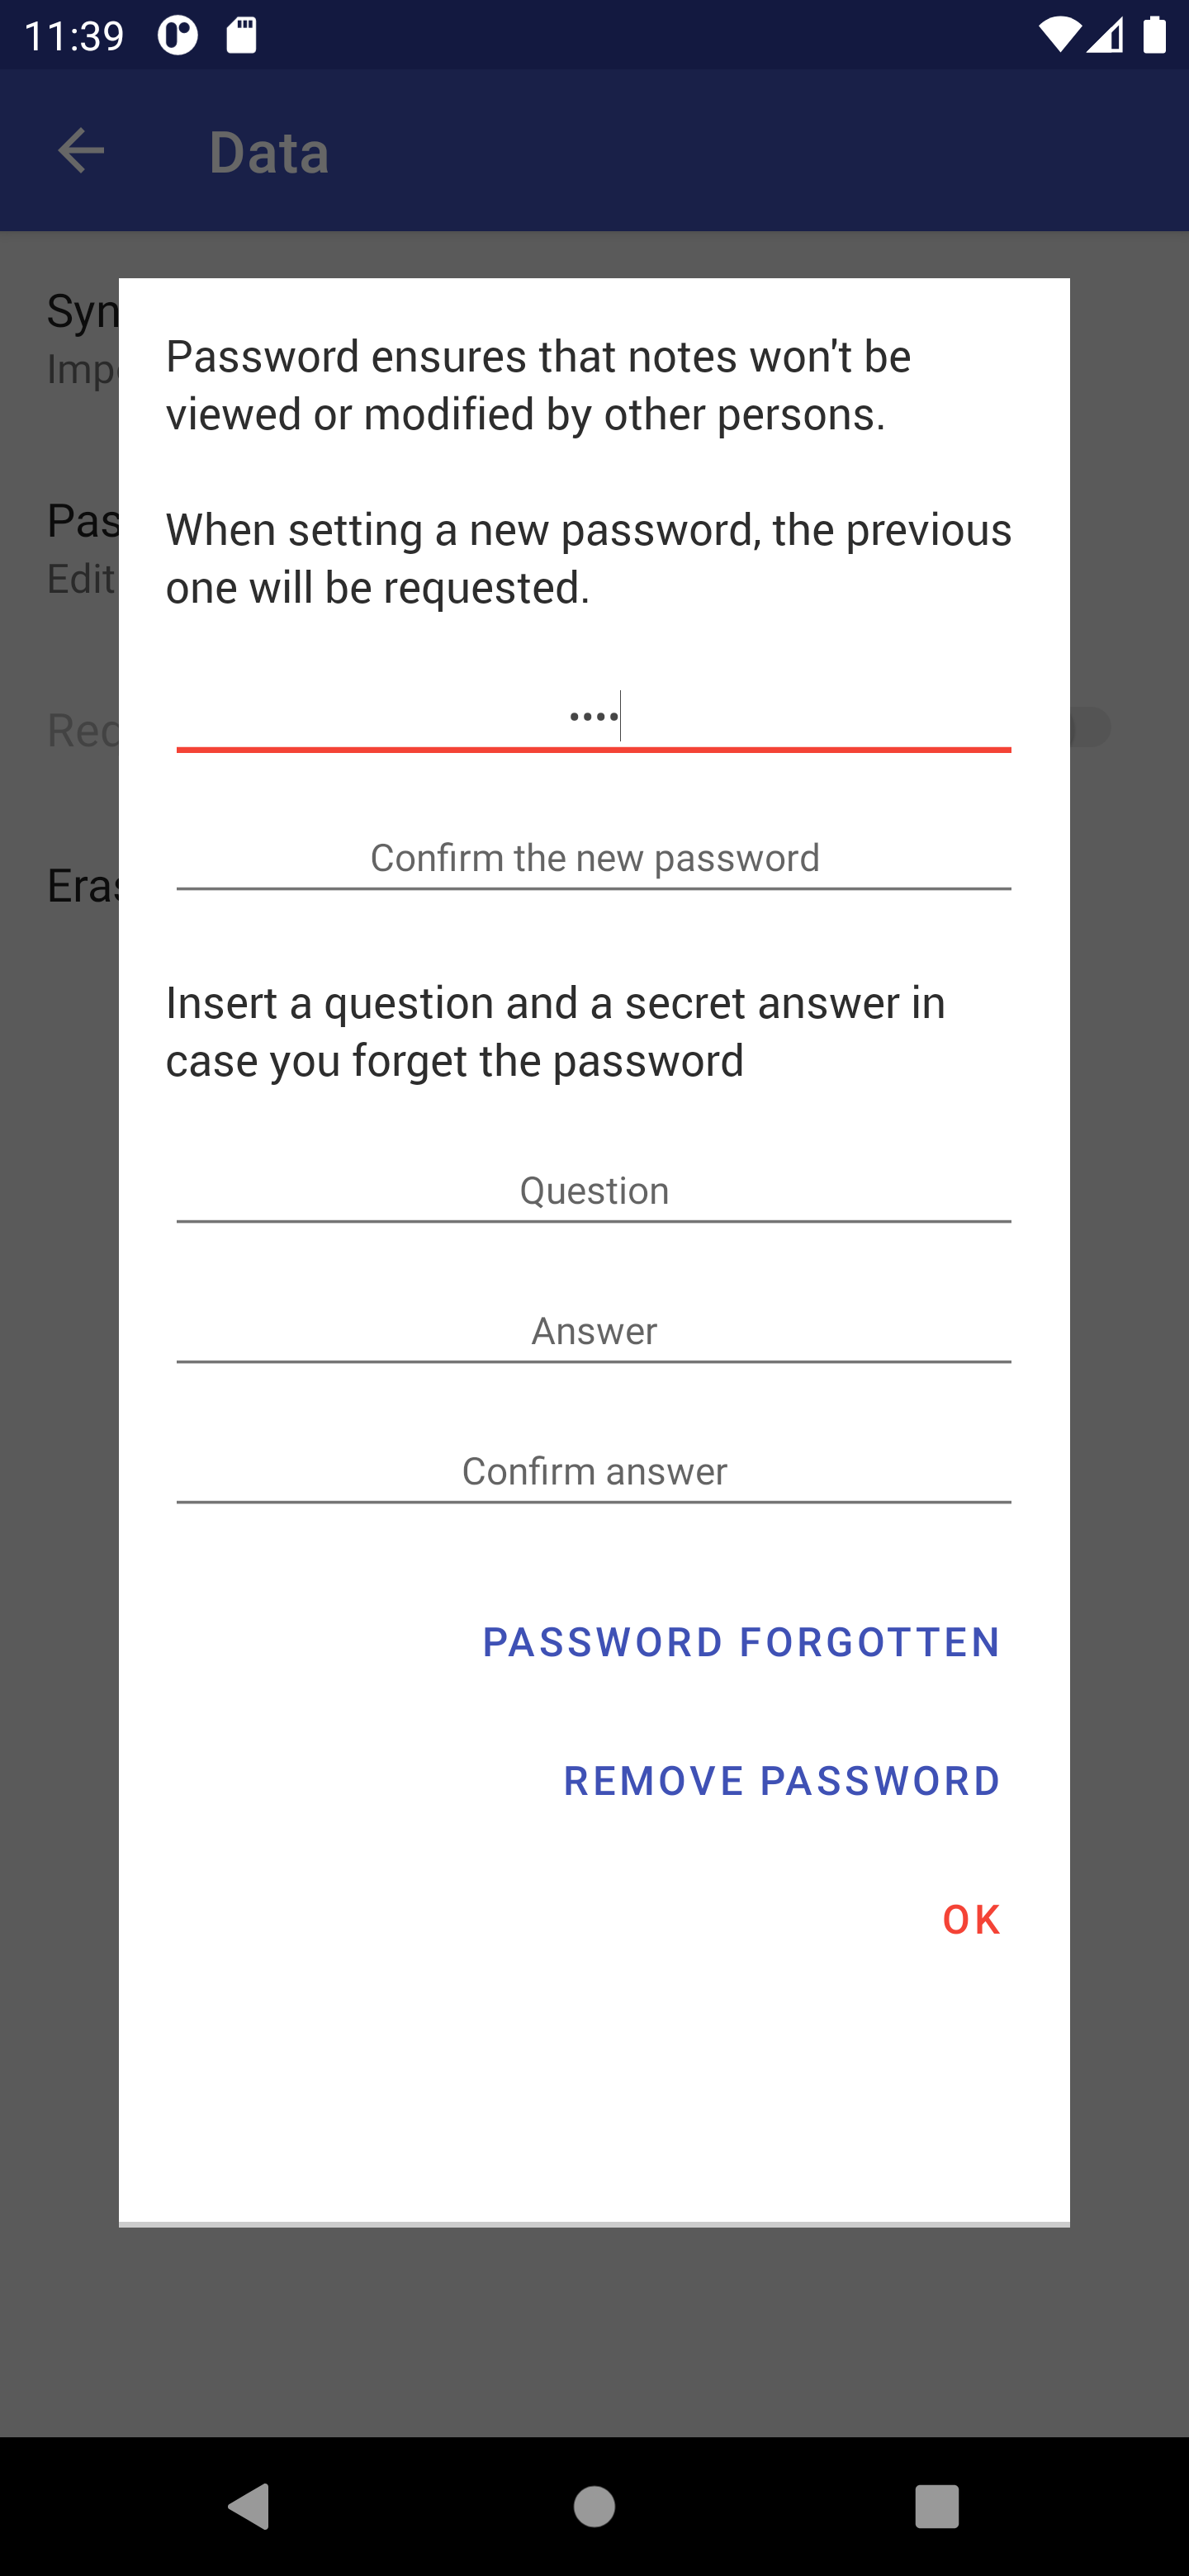
\includegraphics[width=0.8\textwidth]{2.png}
            \caption{Omninotes应用UI陷阱示例}
            \label{fig:ui_trap_example1}
        \end{minipage}
    \hfill
    \begin{minipage}
        [t]{0.4\textwidth}
            \centering
            
\includegraphics[width=0.8\textwidth]{1.png}
            \caption{AnkiDroid应用UI陷阱示例}
            \label{fig:ui_trap_example2}
        \end{minipage}
\end{figure*}

\section{LLM辅助的路径引导策略设计}

为了应对自动探索应用过程中可能遇到的UI陷阱(例如某些界面无响应、需特定操作才能离开、无效路径循环等),本系统引入了大语言模型(LLM)辅助的路径引导机制。具体设计流程如下:

\subsection{策略概述}
在探索过程中,若发现当前UI状态难以探索或无交互反馈,则通过LLM生成用户可能执行的操作序列,用于尝试跳出陷阱状态。这一策略的设计核心是将UI界面的结构(以XML表示)作为上下文输入,利用语言模型生成可能的用户意图与操作,并自动执行以引导状态转移。

\subsection{四级提示工程}


我们设计了四个阶段的提示工程,分别为意图理解阶段、动作生成阶段、校验修正阶段和引导校验阶段。每个阶段的设计旨在引导大语言模型更好地理解当前界面的结构和功能,从而生成更准确的操作序列,以跳出UI陷阱。

\subsubsection{意图理解阶段} 

在这一阶段,我们将获取到的XML结构作为上下文输入到大语言模型中,要求其理解当前界面的意图和功能。我们设计了一个提示词 \texttt{meaning\_prompt()},用于引导模型生成对当前界面的描述。通过获取到模型对当前界面结构的理解,我们可以更好地引导模型生成后续的操作序列。
\begin{lstlisting}[language=Python]
prompt = """This is an XML representation of an Android application page:
{get_xml()}
Please describe the purpose of this page in the most concise language possible."""
\end{lstlisting}

\subsubsection{动作生成阶段} 

在这一阶段,我们将获取到的XML结构和意图描述作为上下文输入到大语言模型中,要求其生成可能的用户操作序列。我们设计了一个提示词 \texttt{action\_prompt()},用于引导模型生成可执行的操作序列。该提示词要求模型输出符合JSON格式的操作序列,并包含必要的属性信息。在这一步中,我们获取到的操作序列以进行后续执行。

\begin{lstlisting}[language=Python]
prompt = """If you were the user, what would you do on this page?
Please provide an action or a sequence of actions in JSON format, for example:
[{{
    "action": "click",
    "selectors": {{"resourceId": "com.example:id/button1"}}
}},
{{
    "action": "input_text",
    "selectors": {{"resourceId": "com.example:id/input", "text": "password"}}
    "inputText": "123456"
}}]
Where:
- action can only be one of: click, long_click, input_text, press, swipe, scroll
- selector can only be one of: text, className, description, resourceId (must be in camelCase); choose the selector that uniquely identifies the element
- the selector's value and must be found in the provided XML
- inputText is the input text, applicable only when action is input_text
- pressKey can be "enter" and applicable only if action is "press"

Please combine multiple selectors to ensure uniquely locating an element.

Before outputting, check whether the value exists in the XML. If it does not exist, modify the action accordingly.

Return only the JSON-formatted action sequence, without explanations or code blocks."""
\end{lstlisting}

\subsubsection{校验修正阶段} 

在这一阶段,我们将获取到的操作序列作为上下文输入到大语言模型中,要求其检查生成的操作序列是否符合要求,以进一步提高操作序列的准确性。我们设计了一个提示词 \texttt{check\_prompt()},用于引导模型检查生成的操作序列是否符合要求。通过这一阶段的校验,我们可以确保生成的操作序列是可执行的,并且在LLM的经验判断下能够有效地跳出UI陷阱。


\begin{lstlisting}[language=Python]
prompt = """Please check whether the operation or sequence of operations you just generated meets the requirements:
- The selector must be found in the XML.
- The selector must uniquely identify the element.
- This sequence of operations must be executable on the current page.
If there are no issues, output it as is; otherwise, modify it accordingly."""
\end{lstlisting}

\subsubsection{最终检查阶段} 

在这一阶段,我们重新获取当前界面的XML结构,并将其作为上下文输入到大语言模型中,要求其判断当前页面是否与前一状态相似。我们设计了一个提示词 \texttt{recheck\_prompt()},用于引导模型判断当前页面是否与前一状态相似。这一阶段的设计旨在避免模型陷入死循环或无响应状态。我们要求模型输出“YES”或“NO”,并根据判断结果生成相应的操作序列。

\begin{lstlisting}
prompt = """Please determine whether the current page is very very similar to the previously displayed XML page.
{get_xml()}
If it is very very similar, find a way to leave the page, output "YES", and then output the operation sequence according to the previous rules.
If it is not similar, output "NO"."""
\end{lstlisting}

\section{实验结果}

为此,我们在不同的应用场景中进行了实验,测试了该策略在不同应用中的表现。我们选择了\textit{AnkiDroid}、\textit{Markor}和\textit{Omninotes}等应用进行测试,并将实验结果与现有的路径引导策略进行了对比分析。我们将实验结果整理成表格,如表\ref{tab:data}和表\ref{tab:pass_percentage}所示。

\begin{table}[h]
    \centering
    \begin{tabular}{lrrr}
        \toprule
        tarpit & old & our & AURORA classify \\
        \midrule
        anki0 & -1 & 1 & 20 Web browser \\
        anki2 & -1 & 1 & 16 Terms and conditions \\
        anki3 & -1 & 1 & 11 Pop up menu \\
        anki4 & 2 & 2 & 13 Search screen \\
        anki5 & 1 & 1 & 13 Search screen \\
        anki6 & 1 & 1 & 11 Pop up menu \\
        anki7 & 1 & 2 & 11 Pop up menu \\
        anki8 & 3 & 1 & 11 Pop up menu \\
        anki9 & -1 & 4 & 4 Form screen \\
        anki10 & 1 & 1 & 18 Type message \\
        markor0 & -1 & -1 & 11 Pop up menu \\
        markor2 & -1 & -1 & 6 List screen \\
        markor6 & -1 & 2 & 11 Pop up menu \\
        ominotes0 & -1 & 1 & 13 Search screen \\
        ominotes2 & 2 & 2 & 6 List screen \\
        ominotes4 & -1 & -1 & 6 List screen \\
        ominotes5 & -1 & 1 & 6 List screen \\
        ominotes6 & -1 & 2 & 6 List screen \\
        ominotes19 & 2 & 1 & 6 List screen \\
        ominotes23 & -1 & 1 & 18 Type message \\
        ominotes25 & -1 & 1 & 16 Terms and conditions \\
        ominotes26 & -1 & 1 & 11 Pop up menu \\
        ominotes28 & 2 & 2 & 18 Type message \\
        ominotes30 & 4 & 1 & 18 Type message \\
        \midrule
        pass & 10 & 21 & \\
        pass/total & 0.4167 & 0.875 & \\
        pass1 & 4 & 14 & \\
        pass1/total & 0.1667 & 0.5833 & \\
        \bottomrule
    \end{tabular}
    \caption{Converted Data Table}
    \label{tab:data}
\end{table}

这个表格中,我们展示了在不同应用中,现有的路径引导策略和我们提出的路径引导策略在处理UI陷阱时的表现。我们将每个应用的测试结果进行了汇总,并计算了通过率。其中,-1表示未能跳出UI陷阱,其余数字表示需要跳出UI陷阱所尝试的次数。我们还采用了Aurora分类器对每个应用进行了分类,并计算了通过率。

\begin{table}[h!]
    \centering
    \begin{tabular}{|l|c|c|c|c|c|}
    \hline
    \textbf{App} & \textbf{All} & \textbf{Filtered} & \textbf{Old} & \textbf{Pass \% (Our)} & \textbf{Pass \% (Other)} \\
    \hline
    Ankidroid & 11 & 10 & 6 & 60 & 100 \\
    Makor & 7 & 3 & 0 & 0 & 33.33 \\
    Ominotes & 31 & 11 & 4 & 36.36 & 90.91 \\
    \hline
    \end{tabular}
    \caption{Pass Percentage Comparison}
    \label{tab:pass_percentage}
    \end{table}

在表\ref{tab:pass_percentage}中,我们展示了在不同应用中,现有的路径引导策略和我们提出的路径引导策略在处理UI陷阱时的通过率对比。我们可以看到,在大多数情况下,我们提出的路径引导策略都能够有效地跳出UI陷阱,而现有的路径引导策略则表现不佳。

\section{总结}

本设计方案提出了一种新的路径引导策略,旨在通过引入更丰富的上下文信息和有效的错误处理机制,来提升操作序列生成的准确性和系统的鲁棒性。我们通过四级提示工程的设计,使得大语言模型能够更好地理解当前界面的结构和功能,从而生成更准确的操作序列。同时,我们也引入了校验机制,以确保生成的操作序列是可执行的,并且能够有效地跳出UI陷阱。在实验数据中,我们将展示该策略在不同应用场景中的表现,并与现有的路径引导策略进行对比分析。

\appendix

\section{附录:完整代码}

\begin{lstlisting}[language=Python]
    import json
    import uiautomator2 as u2
    import xml.etree.ElementTree as ET
    from PIL import ImageDraw
    from openai import OpenAI
    from dataclasses import dataclass
    from IPython.display import display
    from time import sleep, time
    
    from PIL.Image import Image
    from typing import Literal, Optional, cast, ParamSpec, TypeVar, Callable
    from functools import wraps
    
    d = u2.connect()
    d.set_fastinput_ime(True)
    
    gpt_url = ""
    gpt_key = ""
    client = OpenAI(base_url=gpt_url, api_key=gpt_key)
    
    T = TypeVar("T")
    P = ParamSpec("P")
    
    def timer(func: Callable[P, T]) -> Callable[P, T]:
        @wraps(func)
        def wrapper(*args: P.args, **kwargs: P.kwargs) -> T:
            start_time = time()
            result = func(*args, **kwargs)
            end_time = time()
            print(
                f"Execute {func.__name__} in {end_time - start_time:.2f} seconds")
            return result
        return wrapper
    

    def get_xml():
        root = ET.fromstring(d.dump_hierarchy())
    
        flag = False
        for child in root:
            for child_child in child:
                if child_child.attrib['resource-id'] == 'com.android.systemui:id/status_bar_container':
                    root.remove(child)
                    flag = True
                    break
            if flag:
                break
            
        def clean_element(element):
            for attr in list(element.attrib):
                if element.attrib[attr] == "" or element.attrib[attr] == "false":
                    del element.attrib[attr]
            for child in element:
                clean_element(child)
                
        clean_element(root)
    
        res = ET.tostring(root, encoding='unicode')
        res = res.replace("content-desc", "description")
        return res
    
    @timer
    def llm(messages: list):
        response = client.chat.completions.create(
            model="gpt-4o-mini",
            messages=messages,
            temperature=0.7,
        )
        print('>' * 40)
        print(messages[-1]['content'])
        print('<' * 40)
        print(response.choices[0].message.content)
        messages.append({"role": "assistant", "content": response.choices[0].message.content})
        return response.choices[0].message
    

    def meaning_prompt(messages: list):
        prompt = f"""This is an XML representation of an Android application page:
    {get_xml()}
    Please describe the purpose of this page in the most concise language possible.
    """
        messages.append({"role": "user", "content": prompt})
        return messages
    
    def action_prompt(messages: list):
        prompt = f"""If you were the user, what would you do on this page?
    Please provide an action or a sequence of actions in JSON format, for example:
    [{{
        "action": "click",
        "selectors": {{"resourceId": "com.example:id/button1"}}
    }},
    {{
        "action": "input_text",
        "selectors": {{"resourceId": "com.example:id/input", "text": "password"}}
        "inputText": "123456"
    }}]
    Where:
    - action can only be one of: click, long_click, input_text, press, swipe, scroll
    - selector can only be one of: text, className, description, resourceId (must be in camelCase); choose the selector that uniquely identifies the element
    - the selector's value and must be found in the provided XML
    - inputText is the input text, applicable only when action is input_text
    - pressKey can be "enter" and applicable only if action is "press"
    
    Please combine multiple selectors to ensure uniquely locating an element.
    
    Before outputting, check whether the value exists in the XML. If it does not exist, modify the action accordingly.
    
    Return only the JSON-formatted action sequence, without explanations or code blocks.
    """
        messages.append({"role": "user", "content": prompt})
        return messages
    
    
    def check_prompt(messages: list):
        prompt = """Please check whether the operation or sequence of operations you just generated meets the requirements:
    - The selector must be found in the XML.
    - The selector must uniquely identify the element.
    - This sequence of operations must be executable on the current page.
    If there are no issues, output it as is; otherwise, modify it accordingly.
    """
        messages.append({"role": "user", "content": prompt})
        return messages
    
    def recheck_prompt(messages: list):
        prompt = f"""Please determine whether the current page is very very similar to the previously displayed XML page.
    {get_xml()}
    If it is very very similar, find a way to leave the page, output "YES", and then output the operation sequence according to the previous rules.
    If it is not similar, output "NO".
    """
        messages.append({"role": "user", "content": prompt})
        return messages
    

    def parse_recheck(message: str):
        if (message.startswith("YES")):
            message = message[3:]
            return False, message
        return True, None
    
    def error_prompt(messages: list):
        prompt = f"""
    The event sequence you generated encountered an error because the corresponding element could not be found. This is the current XML representation of the application. 
    {get_xml()}
    Correct this error. Output the operation sequence according to the previous rules.
    """
        messages.append({"role": "user", "content": prompt})
        return messages
    
    Selector = Literal['text', 'className',
                          'description', 'resourceId', 'index', 'instance']
    
    @dataclass
    class Action:
        action: Literal['click', 'long_click', 'input_text', 'press', 'swipe', 'scroll']
        selectors: dict[Selector, str]
        inputText: Optional[str] = None
        pressKey: Optional[str] = None
    
    def act(action: Action):
        kwargs = {
            **action.selectors
        }
        
        sc = cast(Image, d.screenshot())
        element = d(**kwargs)
        if element.exists():
            bounds = element.bounds()
            draw = ImageDraw.Draw(sc)
            draw.rectangle(
                bounds,
                outline="red",
                width=5
            )
            draw.text(
                (10, 10),
                action.action,
                fill="red",
                font_size=50
            )
        match action.action:
            case 'click':
                d(**kwargs).click(timeout=0)
            case 'long_click':
                d(**kwargs).long_click(timeout=0)
            case 'input_text':
                d(**kwargs).set_text(action.inputText, timeout=0)
            case 'press':
                d.press('enter')
            case _:
                raise ValueError(f"Unsupported action: {action.action}")
            
        sleep(1)
            
        return sc.resize((int(sc.width / 4), int(sc.height / 4)))
    
    messages = meaning_prompt([])
    llm(messages)
    messages = action_prompt(messages)
    llm(messages)
    messages = check_prompt(messages)
    response = llm(messages)
    actions: list[Action] = [Action(**i) for i in json.loads(str(response.content))]
    
    images = []
    for action in actions:
        try:
            images.append(act(action))
        except:
            messages = error_prompt(messages)
            response = llm(messages)
            new_actions: list[Action] = [Action(**i) for i in json.loads(str(response.content))]
            for action in new_actions:
                images.append(act(action))
        
    sleep(1)
        
    messages = recheck_prompt(messages)
    response = llm(messages)
    
    ok, res = parse_recheck(str(response.content))
    
    if not ok:
        actions = [Action(**i) for i in json.loads(str(res))]
        for action in actions:
            try:
                images.append(act(action))
            except:
                messages = error_prompt(messages)
                response = llm(messages)
                new_actions: list[Action] = [Action(**i) for i in json.loads(str(response.content))]
\end{lstlisting}

\end{document}